\section{Versuchsbeschreibung}

\subsection{Versuchsaufbau}

\begin{figure}[H]
\centering 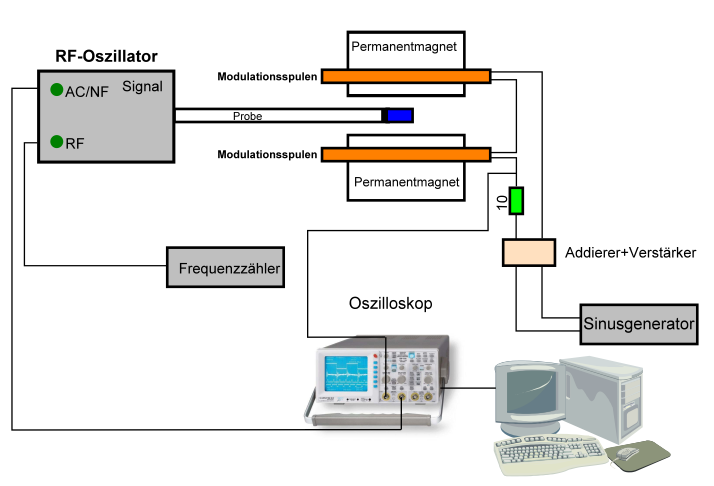
\includegraphics[width= 0.75\textwidth]{Bilder/aufbau1.png}
\caption{Aufbau für den 1. Versuchsteil}
\end{figure}

\begin{figure}[H]
\centering 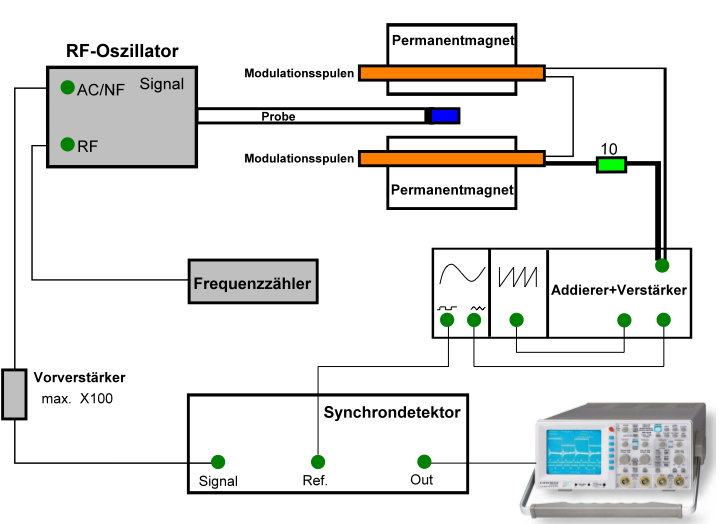
\includegraphics[width=0.75\textwidth]{Bilder/aufbau2.png}
\caption{Aufbau für den 2. Versuchsteil}
\end{figure}

\subsection{Versuchsdurchführung}

Ein Permanentmagnet erzeugt ein homogenes Magnetfeld, welches zusätzlich durch einen Elektromagneten sinusförmig moduliert wird. In das Magnetfeld werden Proben gebracht, welche von einer Spule umgeben sind, die ein hochfrequentes sinusförmiges Feld an der Probe erzeugt. Die Frequenz dieses Feldes wird so eingestellt, dass sie mit jeder Periode zweimal über die Resonanzfrequenz der Probe fährt und somit ein Absorptionssignal am Oszilloskop sichtbar gemacht werden kann. Sind die Absorptionspeaks äquidistant, so tritt die Kernspinresonanz im Nullpunkt des modulierten Magnetfeldes ein, und man kann die eingestellte Frequenz des Spulenfeldes als Resonanzfrequenz des Permanentmagneten ablesen.

\begin{figure}[H]
\begin{minipage}{0.49\textwidth}
\centering 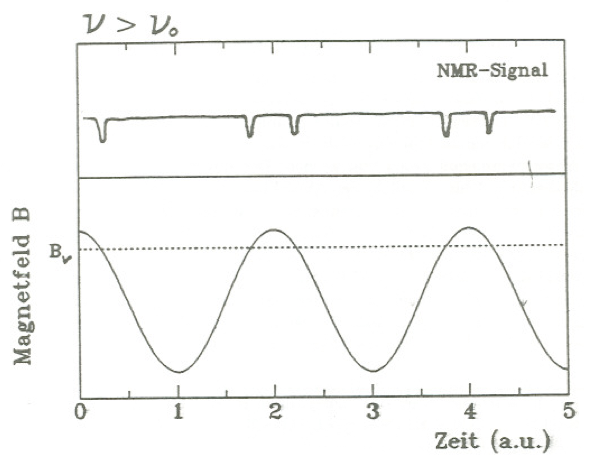
\includegraphics[width=\textwidth]{Bilder/vb1.png}
\end{minipage}
\begin{minipage}{0.49\textwidth}
\centering 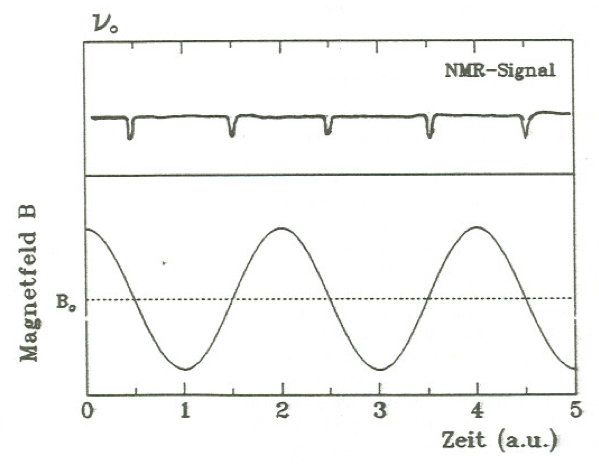
\includegraphics[width=\textwidth]{Bilder/vb2.png}
\end{minipage}
\caption{Absorptionssignale in Abhängigkeit der eingestellten Frequenz}
\end{figure}

Im zweiten Teil des Versuchs modulieren wir das Magnetfeld des Permanentmagneten mit einer Überlagerung aus einer Sägezahnfunktion und einem hochfrequenten Sinus. In der Nähe der Resonanzfrequenz wird die Resonanzstelle im Takt der Modulationsfrequenz überstrichen und das Absorptionssignal ist dementsprechend getaktet. Mit einem Synchrondetektor werden die Resonanzstellen aufgenommen.

\begin{figure}[H]
\centering 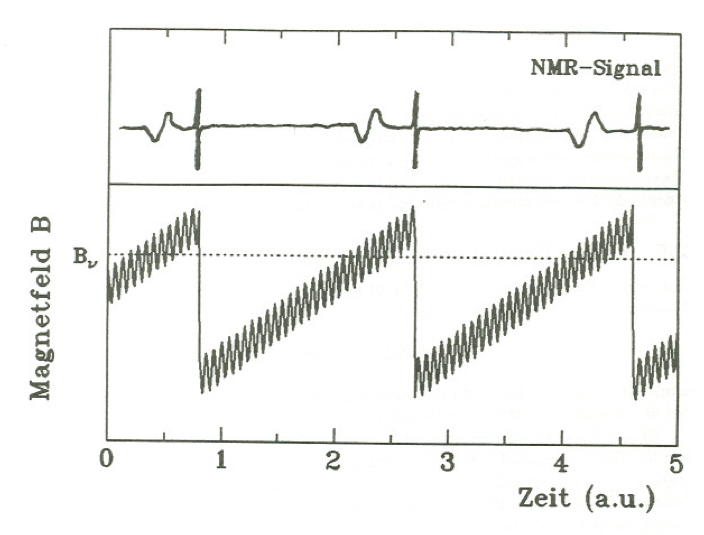
\includegraphics[width=0.5\textwidth]{Bilder/vb3.png}
\caption{Absorption bei Sägezahnmodulation des Magnetfeldes}
\end{figure}